\documentclass[11pt,a4paper]{article}
\usepackage[margin=1in]{geometry}
\usepackage{hyperref}
\usepackage{enumitem}
\usepackage{graphicx}
\usepackage{xcolor}
\usepackage{tikz}
\usetikzlibrary{shapes.geometric, arrows.meta, positioning}

% -----------------------------------------------------
% bvraghav-tiet-ucs503p-article.sty
% -----------------------------------------------------

% Variable: Lab Instructor
\makeatletter \newcommand{\BvrSetLabInstructor}[1]{%
  \gdef\Bvr@LabInstructor{#1}}
% default
\newcommand{\Bvr@LabInstructor}{Dr. Raghav %
  B. Venkataramaiyer}
% public accessor
\newcommand{\BvrLabInstructorValue}{\Bvr@LabInstructor}
\makeatother

% Add subtitle
\usepackage{titling}
% -- Set title bold
\pretitle{\begin{center}\bfseries\fontsize{18bp}{18bp}\selectfont}
\makeatletter
\newcommand{\BvrSubtitle}[1]{%
  \posttitle{%
    \par\end{center}
    \begin{center}\large#1\end{center}
    \vskip 0.5em}%
}
\makeatother

% Hints in the section title(s)
\newcommand{\BvrHint}[1]{%
  {\normalfont\normalsize\itshape\hfill #1}}

% -----------------------------------------------------
\title{\textbf{PRISM}\\[4pt] \large Poverty Risk Identification through Statistical Mapping}
% \title{PRISM}
\BvrSetLabInstructor{Dr. Raghav B. Venkataramaiyer}

\BvrSubtitle{%
  Project Proposal for UCS503  \\
  Submitted to: \BvrLabInstructorValue \\ \bfseries
  Thapar Institute of Engineering and Technology% 
}

\author{
  Amish Kapoor, CSED%
  \thanks{Roll No: \texttt{1024160005}, %
    Email: \texttt{akapoor\_be24\@thapar.edu}}
  \and 
  Aryan Chaturvedi, CSED%
  \thanks{Roll No: \texttt{1024160009}, %
    Email: \texttt{achaturvedi1\_be24\@thapar.edu}}
  \and 
  Kushal, CSED%
  \thanks{Roll No: \texttt{1024160003}, %
    Email: \texttt{kkushal\_be24\@thapar.edu}}
}

\date{\today}

\begin{document}
\maketitle

\section{Higher-order goal%
  % \BvrHint{\ldots secondary framing}
  }
This project aims to close the gap between where India's development funds and interventions actually go, and where they are most urgently needed. Despite running some of the world's largest anti-poverty programmes, resource allocation still leans heavily on outdated, single-source indicators — mainly Census 2011 — while newer, richer data streams like the SDG India Index and NFHS remain siloed and underused. While the topic is broader than any single ministry or scheme, the immediate engineering objective is to translate scattered, unvalidated development data into a measurable, explainable, and policy-actionable classification of district-level need.

\section{Time-to-value %
% \BvrHint{\ldots primary heuristic}
}
\begin{itemize}[leftmargin=0.7cm]
    \item We will deliver meaningful increments quickly by checking our early district classifications against the government's own Aspirational Districts Programme list, giving us an honest signal on whether the approach works before investing further effort.
    \item We will prioritize validation over polish by testing whether our model's output could plausibly justify a real intervention decision, rather than chasing marginal accuracy gains on an unverified classification pipeline.
    \item Success is defined not by accuracy alone, but by whether the model can explain why a district is flagged as under-developed, not just that it is, since only that makes it policy-actionable.
\end{itemize}

\section{Problem Statement}
Policymakers assessing district-level poverty in India face outdated data and unclear accountability when deciding where interventions are needed most. Common pain points include:
\begin{itemize}[leftmargin=0.7cm]
    \item \textbf{Outdated snapshots:} major assessments still lean on Census 2011, over a decade old, missing shifts newer surveys have already captured.
    \item \textbf{Fragmented indicators:} health, income, and infrastructure data live in separate government sources, so no single study sees the full picture.
    \item \textbf{No ground-truth check:} classifications are rarely validated against a real outcome, such as the government's own Aspirational Districts list.
    \item \textbf{No explanation, only a label:} models flag districts as at-risk without saying why, leaving no basis for targeted action.
\end{itemize}

\textbf{Why this matters now (contextual relevance):} With India's largest anti-poverty programmes needing measurable, data-backed evidence of real impact, an outdated or unvalidated classification can misdirect resources meant for the districts that need them most urgently.

\section{Proposed Solution %
% \BvrHint{\ldots Software Proposition}
}
\subsection{Overview}
Build a data-driven ``Poverty-Zone Identification'' system with the following components:
\begin{itemize}[leftmargin=0.7cm]
    \item \textbf{Data fusion layer:} merge SDG India Index, Census 2011, and NFHS-5 into a single district-level dataset using cleaned state/district keys.
    \item \textbf{Clustering module:} group districts by development level using K-Means and hierarchical clustering, unsupervised and label-free.
    \item \textbf{Classification module:} predict Aspirational-District status using Logistic Regression, Random Forest, SVM, and other classifiers, benchmarked against each other.
    \item \textbf{Explainability layer:} surface feature importance (via Random Forest) so each classification comes with a reason, not just a label.
    \item \textbf{Validation check:} compare model output against the real Aspirational Districts Programme list to confirm results are grounded in fact.
\end{itemize}

\subsection{Core workflow}
\begin{enumerate}[leftmargin=0.7cm]
    \item Raw district data is collected from SDG Index, Census, and NFHS sources.
    \item District names are cleaned and matched across sources to enable a reliable merge.
    \item The fused dataset is scaled and clustered to group districts by development level.
    \item Classifiers are trained on the fused data and evaluated against the Aspirational Districts list.
    \item Feature importance is extracted so each flagged district's classification is explainable.
\end{enumerate}

\subsection{Operational constraints for an educational, tier-2/3 setting}
\begin{itemize}[leftmargin=0.7cm]
    \item Keep the pipeline reproducible on standard laptops using Python (Pandas, scikit-learn); avoid dependence on proprietary or paid data tools.
    \item Avoid dependence on satellite imagery or deep learning pipelines; focus on tabular government data and classical ML, matching syllabus scope.
    \item Design for a demoable output — a simple dashboard or notebook that a non-technical evaluator can follow end-to-end.
\end{itemize}

\section{Solution Approach %
% \BvrHint{\ldots Engineering focus}
}
\begin{figure}[h]
\centering
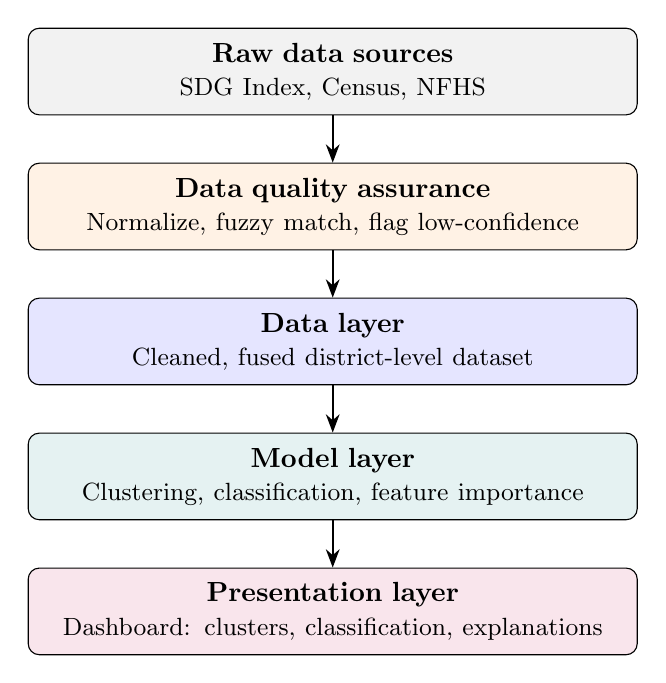
\begin{tikzpicture}[
    node distance=0.6cm,
    box/.style={rectangle, rounded corners, draw, fill=gray!10,
                text width=7.5cm, align=center, minimum height=1.1cm},
    arr/.style={-Stealth, thick}
]
\node[box] (raw) {\textbf{Raw data sources}\\ \small SDG Index, Census, NFHS};
\node[box, below=of raw, fill=orange!10] (dqa) {\textbf{Data quality assurance}\\ \small Normalize, fuzzy match, flag low-confidence};
\node[box, below=of dqa, fill=blue!10] (data) {\textbf{Data layer}\\ \small Cleaned, fused district-level dataset};
\node[box, below=of data, fill=teal!10] (model) {\textbf{Model layer}\\ \small Clustering, classification, feature importance};
\node[box, below=of model, fill=purple!10] (pres) {\textbf{Presentation layer}\\ \small Dashboard: clusters, classification, explanations};

\draw[arr] (raw) -- (dqa);
\draw[arr] (dqa) -- (data);
\draw[arr] (data) -- (model);
\draw[arr] (model) -- (pres);
\end{tikzpicture}
\caption{Solution approach: data fusion and processing pipeline}
\label{fig:solution-pipeline}
\end{figure}

\subsection{Data quality assurance %
% \BvrHint{\ldots non-research}
}
District matching across sources will be rule-based:
\begin{itemize}[leftmargin=0.7cm]
    \item Normalize district and state names (lowercase, strip "district"/"dist." suffixes) before any merge.
    \item Use a simple similarity measure (e.g., fuzzy match with a confidence threshold) without claiming state-of-the-art matching.
    \item Flag low-confidence matches for manual review; never auto-merge a district without a check.
\end{itemize}

\subsection{System architecture %
% \BvrHint{\ldots web-based solution}
}
A typical 3-layer data pipeline:
\begin{itemize}[leftmargin=0.7cm]
    \item \textbf{Data layer:} cleaned, fused district-level dataset combining SDG Index, Census, and NFHS records.
    \item \textbf{Model layer:} clustering, classification, and feature-importance modules built with scikit-learn.
    \item \textbf{Presentation layer:} dashboard or notebook showing district clusters, classification results, and explanations.
\end{itemize}

\subsection{Reproducibility and fast delivery enabler}
Scripted, version-controlled pipelines will be used to:
\begin{itemize}[leftmargin=0.7cm]
    \item Automatically re-run preprocessing and model training whenever source data is updated.
    \item Produce reproducible, versioned outputs for every experiment and model comparison.
    \item Enable fast iteration across clustering and classification approaches without manual rework.
\end{itemize}

\section{Evaluation Criterion %
% \BvrHint{\ldots measurable and attributable}
}
We define success using measurable metrics tied to real government outcomes.

\subsection{Primary evaluation metric}
\textbf{Validation agreement with Aspirational Districts:} overlap between model-predicted under-developed districts and the government's official Aspirational Districts list.
\begin{itemize}[leftmargin=0.7cm]
    \item Target: at least 75\% overlap with the official list during initial validation.
    \item Attribution: measured via precision and recall against the 112-district ADP ground truth.
\end{itemize}

\subsection{Secondary evaluation metrics}
\begin{itemize}[leftmargin=0.7cm]
    \item \textbf{Clustering quality:} silhouette score of district clusters formed from the fused dataset.
    \item \textbf{Classification robustness:} F1-score compared across Logistic Regression, Random Forest, SVM, and other classifiers.
    \item \textbf{Explainability coverage:} proportion of flagged districts with a clear top-3 feature explanation.
    \item \textbf{Data completeness:} percentage of districts successfully matched across all fused sources.
\end{itemize}

\subsection{Validation plan %
% \BvrHint{\ldots high-level}
}
\begin{itemize}[leftmargin=0.7cm]
    \item Test the pipeline on 2–3 states first, mixing high- and low-development regions, before scaling nationally.
    \item Compare model-flagged districts against the Aspirational Districts list and log mismatches for review.
\end{itemize}

\section{Scalability %
% \BvrHint{\ldots with foresight}
}
The proposition should scale in both theoretical and practical senses.

\begin{enumerate}[leftmargin=0.7cm]
    \item \textbf{Scalable (theoretically):} The system should support growth in number of districts, indicators and data sources by:
    \begin{itemize}[leftmargin=0.7cm]
        \item decoupling the data-fusion layer from the modeling layer,
        \item enabling incremental re-clustering as new districts or survey years are added,
        \item using a modular pipeline where new datasets plug in without rewriting existing code.
    \end{itemize}
    
    \item \textbf{Operationally deployable (practically):} The pipeline should run using common tools:
    \begin{itemize}[leftmargin=0.7cm]
        \item standard Python data-science stack (Pandas, scikit-learn),
        \item version-controlled scripts for reproducible re-runs,
        \item lightweight scheduling (e.g., a single command or notebook run) for staging updated data.
    \end{itemize}
\end{enumerate}

\section{Technology Stack}
A mature set of open, well-documented tools is available to implement this as a data-driven analysis project:
\begin{itemize}[leftmargin=0.7cm]
    \item Data manipulation library for merging and cleaning district-level datasets (Pandas).
    \item Established clustering and classification library (scikit-learn) covering K-Means, Random Forest, SVM, and more.
    \item Visualization library for cluster maps and feature-importance charts (Matplotlib/Seaborn).
    \item Fuzzy string-matching library for district name reconciliation across sources.
    \item Notebook or lightweight dashboard framework for presenting results to a non-technical evaluator.
    \item Version control (Git) for tracking preprocessing decisions and model iterations.
\end{itemize}
We will use these mature components to focus on data fusion, validation, and explainability rather than building modeling infrastructure from scratch.

\section{Project scope and deliverables %
% \BvrHint{\ldots iteration-friendly}
}
\subsection{Initial deliverable %
% \BvrHint{\ldots first iteration}
}
\begin{itemize}[leftmargin=0.7cm]
    \item Data fusion script: merge SDG Index, Census, and NFHS into one district table
    \item District name matching: cleaned and validated state/district keys across sources
    \item K-Means clustering: initial development-tier grouping of districts
    \item Basic evaluation: cluster overlap check against the Aspirational Districts list
    \item CI: automated tests for data merge correctness + linting
    \item CD to staging with a single command or pipeline job
\end{itemize}

\subsection{Subsequent deliverables}
\begin{itemize}[leftmargin=0.7cm]
    \item Additional classifiers (Random Forest, SVM, Naïve Bayes) with performance comparison
    \item Feature-importance layer for explainable classification results
    \item Hierarchical clustering as a cross-check against K-Means results
    \item Dashboard or notebook view for district-level exploration and results
    \item Expanded validation across more states for robustness
\end{itemize}

\section{Risks and mitigations}
\begin{itemize}[leftmargin=0.7cm]
    \item \textbf{Data mismatch risk:} district names differ across sources; mitigate with rule-based cleaning plus manual review of low-confidence matches.
    \item \textbf{Ground-truth ambiguity:} the Aspirational Districts list uses its own undisclosed criteria; mitigate by treating it as a directional check, not an exact target.
    \item \textbf{Feature imbalance:} flagged districts are a minority class; mitigate using precision/recall over raw accuracy during evaluation.
    \item \textbf{Scope creep in modeling:} too many algorithms could stall progress; mitigate by locking a baseline model early and adding others incrementally.
\end{itemize}

\section{Summary}
This project proposes a fused, validated, and explainable machine learning pipeline to identify poverty and development zones across Indian districts. It meets the course criteria by emphasizing reproducibility through versioned preprocessing, validating results against real government outcomes, and using measurable evaluation criteria (especially agreement with the Aspirational Districts list). It remains focused on data-engineering rigor and explainability rather than novel model architecture.

\end{document}
